\documentclass[fr]{../../../eplsummary}

\usepackage{graphicx}
\usepackage{enumerate}
\usepackage{standalone}
\usepackage{listings}
\usepackage{float}
\usepackage{caption}
\usepackage{rotating}
\usepackage{booktabs}
\usepackage{lscape}
\usepackage{framed}
\usepackage[disable, colorinlistoftodos]{todonotes}
\usepackage{chngcntr}
\usepackage{geometry}
\usepackage[bottom]{footmisc}
\usepackage{wrapfig}
\geometry{hmargin=1.8cm, vmargin=1.8cm}
\usepackage[american]{circuitikz}
\usepackage{adjustbox}

\setcounter{tocdepth}{2}
\counterwithin{figure}{section}

% -------- MACROS -----------------
\newcommand{\Lagr}{\mathcal{L}} % signe lagrangien
\newcommand{\EvalAt}[1]{\biggr\rvert_{#1}} % pour faire la barre d'evaluation en un point (p. ex. \EvalAt{x=0}
\newcommand{\Module}[1]{\vert #1 \vert} % pour la valeur absolue/module (p. ex. \Module{x}
\newcommand{\Argex}[1]{e^{#1 j}} % pour expo avec angle dedans
\newcommand{\Polar}[2]{\Module{#1}\Argex{#2}} % pour une notation polaire rapide (p. ex. \Polar{V_{max}}{\phi}
% J'aurais dû faire un macro pour les \stackrel{\triangle}{=} :'(

\hypertitle{Circuits \& Mesures}
{4}{ELEC}{1370}
{Philippe Greiner\and Vincent Schellekens}
{Francis Labrique et Charles Trullemans}

\listoftodos
\newpage

\section{Circuits résistifs et ampli op}
\subsection{Notions de base : rappels et conventions}
\subsubsection{Loi de Ohm}
La loi de Ohm relie la tension et le courant sur une résistance est simplement donnée par $\boxed{v(t) = R\cdot i(t)}$, où $R\ge 0$. On rappelle aussi la notion de \textbf{conductance}, avec $G = \frac{1}{R}$. Avec la conductance, la loi de Ohm est $v(t) = \frac{i(t)}{G}.$
\paragraph{Puissance} On définit la puissance (instantanée) comme $p(t) = v(t) \cdot i(t)$\footnotemark. Dans le cas de la résistance, on peut facilement utiliser la loi de Ohm pour obtenir $p(t) = R\cdot i^2(t) = \frac{v^2(t)}{R}$.
\footnotetext{Il est important de définir le courant et la tension sur le circuit de \textbf{directions opposées} pour cette formule, pour ne pas en changer le signe: le courant entre dans une résistance du côté \textbf{positif} à la borne positive de tension.}

\subsubsection{Kirchoff}
On rappelle brièvement les deux lois de Kirchoff, indispendables pour la résolutions de circuits.
\paragraph{Loi des noeuds (KCL)}
La loi des noeuds, ou loi des courants, s'écrit $\sum^{N}_{j=1}i_j(t) = 0$: la somme de tous les courants en un noeud est nulle. Les courants doivent être soit tous divergents, soit convergents.
\paragraph{Loi des mailles (KVL)}
La loi des mailles s'exprime sur les tensions, et se formule de la manière suivante: $\sum^N_{j=1}v_j(t) = 0$, où les tensions sont prises dans une boucle fermée\footnote{On appelle boucle fermée tout parcours fermé dans le circuit, tel qu'aucun noeud n'est rencontré deux fois.} du circuit.
\subsubsection{Résolution de circuits}
Voici quelques cas typiques qui permettront de résoudre efficacement des circuits plus compliqués par la suite.
\paragraph{Résistances en parallèle}
Pour additioner plusieurs résistances branchées en parallèle, on a $\frac{1}{R_{eq}} = \frac{1}{R_1} + \dots + \frac{1}{R_n}$, ce qui donne $R_{eq} = \frac{R_1\ldots R_n}{R_1+\ldots+R_n}.$
\paragraph{Diviseur de tension}
Figure \ref{diviseurs} à gauche: la tension dans la résistance $R_1$ est de $v_{R_1} = v(t)\cdot\frac{R_1}{R_1+R_2}.$
\paragraph{Diviseur de courant}
Figure \ref{diviseurs} à droite: le courant dans la résistance $R_1$ est de $i_{R_1} = i(t)\cdot\frac{R_2}{R_1+R_2}.$
\begin{figure}[H]
\centering
\begin{circuitikz}[american]
\draw (0,0) to [V = v(t)] (0,2) to[R=$R_1$] (2,2) to[R=$R_2$] (2,0) -- (0,0); 
\draw (5,0) to [I = i(t)] (5,2) -- (6,2) to [R=$R_1$,*-*] (6,0) -- (5,0);
\draw (6,2) -- (7.5,2) to [R=$R_2$] (7.5,0) -- (6,0);

\end{circuitikz}
\caption{Diviseur de tension (à gauche) et de courant (à droite)}
\label{diviseurs}
\end{figure}

\paragraph{Equivalence étoile $\longleftrightarrow$ triangle}
Comme visible à la figure \ref{triangle}, il est aisé de convertir un triangle, en gardant les mêmes bornes. Cela facilitera grandement la résolution des circuits en triangles, en rendant les lois de Kirchoff plus facilement applicables.
Pour passer de triangle à étoile, on remplace\footnotemark\ deux résistances($R_1$ et $R_2$) connectées à un même pôle par une seule résistance $$R_a = \frac{R_1\cdot R_2}{R_1+R_2+R_3}$$ connectée à ce même pôle. Pour la transformation inverse (beaucoup moins utile), on a $R_1 = \frac{R_aR_b + R_bR_c + R_aR_c}{R_b}$.
\footnotetext{La démonstration n'est pas donnée ici, mais il suffit d'égaler les résistances équivalentes entre chaque borne puis de résoudre.}
\begin{figure}[H]
\centering
\begin{circuitikz}[american]
	\draw (0,0) node[left]{c} to[R=$R_1$,*-*] (2,2.82)node[above]{a} to[R=$R_2$,-*] (4,0) node[right]{b} to[R=$R_3$] (0,0); 
	\draw (6,0) node[left]{a} to[R=$R_1$,-*](8,0.94);
	\draw (8,2.82) node[above]{b} to[R=$R_2$](8,0.94);
	\draw (10,0) node[right]{c} to[R=$R_3$](8,0.94);
\end{circuitikz}
\caption{Circuit en triangle et en étoile}
\label{triangle}
\end{figure}
\paragraph{Principe de superposition} Le principe de superposition dit que la réponse dans une branche est égale à la somme des réponses pour chaque générateur indépendant pris isolément, en annulant tous les autres générateurs indépendants. Pour annuler une source, on remplace une source de tension par un court circuit et une source de courant par un circuit ouvert.

\subsection{Amplificateur opérationnel : modèle idéal}
\begin{figure}[h]
\centering

\begin{circuitikz}[american]
	\draw (0,0) node[op amp] (op){};
	\draw (op.-) -- ++(-0.2,0) -- ++ (0,1) -- ++ (2.58,0) -- (op.out);
	\draw (op.+) ++(-1,-1.5) node[ground]{} to[V=$V_s$] ++(0,1.5) -- (op.+);
	\draw (op.out) -- ++(0.5,0) node[right]{$V_o$};
	
	\draw (4,-1) node[ground]{} to[V=$V_s$] (4,1) -- ++(1.5,0) to[R=$R_1$,v=$V_{in}$] ++(0,-1.75) -- ++(1,0)--++(0,1.75)--++(2,0) -- ++ (0,-1) -- ++(0.5,0)node[right]{$V_o$};
	\draw (7,-2.5)node[ground]{} to[american controlled voltage source=$A_oV_{in}$] ++(0,2.5) to[R=$R_o$,-*] ++(1.5,0);
\end{circuitikz}

\caption{Amplificateur opérationnel: buffer à gain unitaire et modèle d'ampli op}
\label{fig:aop}
\end{figure}

\begin{figure}[h]
	\centering
	
	\begin{circuitikz}[american]
		\draw (4,1)node[left]{$IN_+$} -- ++(1.5,0) to[R=$R_1$,v=$V_{in}$] ++(0,-1.75) -- ++(-1.5,0) node[left]{$IN_-$};
		\draw (7,-2.5)node[ground]{} to[american controlled voltage source=$A_oV_{in}$] ++(0,2.5) to[R=$R_o$] ++(1.5,0)--++(0.5,0)node[right]{$V_o$};
	\end{circuitikz}
	
	\caption{Amplificateur opérationnel idéal}
	\label{fig:aopgen}
\end{figure}
Sur la figure \ref{fig:aop}, le circuit de gauche est un montage basique avec un amplificateur opérationnel. Le circuit à droite représente un modèle équivalent au circuit. Plus précisément, on représente un amplificateur opérationnel (figure \ref{fig:aopgen}) par\footnote{Pour l'instant du moins, on parlera plus tard de certaines non idéalités} une résistance $R_i$ entre les bornes à l'entrée, et une source commandée par la tension aux bornes de cette résistance $V_{in}$ (avec un gain $A_o$), en série avec une résistance de sortie $R_o$. La relation entre tension d'entrée et de sortie est, d'après le modèle, donnée par $$\frac{V_o}{V_s} = \cfrac{1}{1+\cfrac{R_i}{R_o + A_oR_i}}.$$
Pour obtenir le modèle de l'amplificateur opérationnel idéal, on va faire les approximations suivantes:
$$\left\{ \begin{array}{c}
A_o \longrightarrow \infty\\
R_i \longrightarrow \infty\\
R_o \longrightarrow 0
\end{array}\right. $$

Avec ces approximations, on observe un gain de 1 pour ce circuit. Les conséquences pratiques pour la résolution de circuits avec ce modèle idéal (montré à la figure \ref{fig:aopIO}) sont $\boxed{i_+ = i_- = 0}$ et $\boxed{v_+ = v_-}$. Ces simplifications seront extrèmement pratiques pour les circuits.

\begin{figure}[h]
\centering
\begin{circuitikz}[american]
	\draw (0,0) node[op amp] (op){};
	\draw (op.-) ++ (-1,0) to[short,i=$i_-$] (op.-)node[above]{$V_-$};
	\draw (op.+) ++ (-1,0) to[short,i_=$i_+$] (op.+) node[below]{$V_+$};
	\end{circuitikz}
\caption{Conventions de sens pour l'amplificateur opérationnel.}
\label{fig:aopIO}
\end{figure}

\subsection{Dipôles équivalents}
\label{dipoles}
\todo[inline,color=blue]{Revoir éventuellement comment on introduit le bazar}
Tout circuit contenant des résistances\footnote{Plus tard, on verra que c'est aussi vrai pour un circuit contenant tout types d'impédances. Dans ce cas, la résistance équivalente $R_{Th}$ est remplacée par une impédance équivalente $Z_{Th}$.} et des sources (on parle alors d'un \textit{circuit résistif}) peut être remplacé par un \textbf{dipôle équivalent de Norton ou de Thévenin} : les caractéristiques du circuit vues par \textit{l'extérieur} du circuit sont alors préservées. Le dipôle équivalent est constitué d'une source équivalente (de tension ou de courant) et d'une \textbf{résistance équivalente} $R_{Th}$.  Cela permet de simplifier grandement une partie du circuit qui ne nous intéresse pas beaucoup. Par exemple, si on étudie un circuit comportant une inductance et qu'on s'intéresse au courant passant par cette inductance, on peut construire le circuit équivalent aux bornes de celle-ci.



\begin{figure}[h]
	\centering
    \begin{circuitikz}
    	\draw (0,0) rectangle (2,3);
    	\draw (1,1.5)node[align = center]{Circuit\\complexe};
    	\draw (2,2.5) -- (2.5,2.5) node[right]{A};
    	\draw (2,0.5) -- (2.5,0.5) node[right]{B};
    	\draw (6,3) -- (4,3) to[V=$V_{oc}$] (4,5) to[R=$R_{th}$] (6,5) to[open,*-*,v=$v_o$] (6,3);
    	\draw (7,-2) -- (4,-2) to[I=$I_{sc}$] (4,0) -- (6,0) to[R,l_=$R_{th}$,*-*] (6,-2);
    	\draw (6,0) -- (7,0) to[open,*-*,v=$v_o$] (7,-2);
    	\draw [thick,latex-latex] (5, 2.5) -- (5,0.5) node[midway,right]{$V_{oc} = R_{th} I_{sc}$};
    \end{circuitikz}
    \caption{Equivalents de Thévenin (droite, haut) et Norton (droite, bas).}
     \label{thev}
\end{figure}

On parle d'\textbf{équivalent Thévenin} (en haut à droite de la figure \ref{thev}) si on a une source de tension $V_{OC}$. Cette tension $V_{OC}$ est la tension mesurée aux bornes du circuit à simplifier en circuit ouvert\footnote{\og Open Circuit\fg}. La résistance $R_{Th}$ est alors placée en série avec la source de tension. Par contre, dans un \textbf{équivalent de Norton} (en bas à droite de la figure \ref{thev}), la source est une source de courant $I_{SC}$, qui est le courant mesuré aux bornes du circuit en court circuit (on connecte les deux bornes du circuit)\footnote{\og Short Circuit\fg}. $R_{Th}$ est alors placée en parallèle avec la source. ATTENTION : la résistance $R_{Th}$ est la même dans les deux cas! On peut facilement passer de l'un à l'autre grâce à la relation :
\begin{equation}
V_{OC} = R_{Th}I_{SC}
\end{equation}

En pratique, comment construire un équivalent? Grâce à l'équation ci-dessus, il suffit de déterminer deux des trois grandeurs $V_{OC}$, $I_{SC}$ et $R_{Th}$ pour construire n'importe quel équivalent. Il est parfois plus intéressant de par exemple calculer $I_{SC}$ et $R_{Th}$ même si on construit l'équivalent Thévenin, si $I_{SC}$ est plus facile à déterminer.

\paragraph{Trouver $V_{OC}$} : on prend le circuit compliqué isolé, et on calcule la tension entre les bornes (qui sont en circuit ouvert).

\paragraph{Trouver $I_{SC}$} : de manière similaire, on prend le circuit compliqué isolé, on connecte les bornes par un simple fil, et on calcule le courant à travers ce fil.

\paragraph{Trouver $R_{Th}$} : ici la stratégie est plus subtile, car elle dépend des sources présentes dans le circuit.
\begin{itemize}
\item \textbf{Que des sources indépendantes} : $R_{Th}$ peut être évalué en annulant les sources\footnote{Une source de tension est remplacée par un fil, assurant une tension nulle, et une source de courant par un "trou", assurant un courant nul.}, puis en déterminant la résistance équivalente aux bornes du circuit. Bien sûr, si on veut, on peut toujours utiliser $R_{Th} = V_{OC}/I_{SC}$.
\item \textbf{Sources dépendantes + indépendantes} : il faut obligatoirement, sauf cas particulier\footnote{Si on est certain que les sources dépendantes s'annulent si les sources indépendantes sont nulles.}, utiliser $R_{Th} = V_{OC}/I_{SC}$ si il y a des sources dépendantes. Cela provient du fait qu'on ne peut pas annuler arbitrairement une source dépendante sans être certain que la variable qui la contrôle est nulle aussi.
\item \textbf{Que des sources dépendantes} : il faut utiliser une source "test" (par exemple d'un volt) que l'on place aux bornes du circuit. On peut ensuite calculer la résistance équivalente du circuit qui est égale à la tension aux bornes de la source test sur le courant passant par la source test. Remarquons aussi que dans le cas d'un circuit comportant uniquement des sources dépendantes, la source équivalente est toujours nulle (car il n'y a pas de source d'énergie dans le circuit isolé) et le dipôle équivalent se réduit toujours à une simple résistance.
\end{itemize}

\section{Analyse AC (1) : solutions sinusoïdales en régime (alias les phaseurs)}
\subsection{Rappels : capacité et inductance}
Avant d'introduire les phaseurs, voici un rapide rappel des circuits RC et RL de premier ordre. Pour obtenir la solution dans ces circuits, on doit résoudre une équation différentielle. A tout hasard, on rappelle aussi que
\begin{align}
\text{Capacité: }& i(t) = C\cdot \frac{dv(t)}{dt}\label{C}\\
\text{Inductance: }& v(t) = L\cdot \frac{di(t)}{dt}\label{L}
\end{align}



\begin{figure}[H]
\centering
\begin{circuitikz}[american]
	\draw (0,0) to[V=$V_s$] (0,2.5) to[R=R,v=$V_R$] (2.5,2.5) to[C=C,v=$V_C$] (2.5,0)-- (0,0);
	\draw (4.5,0) to[I=$I_s$] (4.5,2.5) -- (5.5,2.5) to[R=R,i=$I_R$,*-*] (5.5,0) -- (4.5,0);
	\draw (5.5,2.5) -- (6.5,2.5) to[L=L,i=$I_L$] (6.5,0) -- (5.5,0);
\end{circuitikz}
\caption{Circuit RC (à gauche) et RL (à droite)}
\label{RCRL}
\end{figure}

A la figure \ref{RCRL}, on voit les deux circuits de base avec une capacité et une résistance.
On commence par résoudre le circuit RC (à gauche). En appliquant KVL, on a
\begin{align}
V_s(t) = V_R(t) + V_C(t) \label{VRC}
\end{align}
Le circuit étant en série, on a le même courant partout, qui vaut
\begin{align}
I(t) = \frac{V_R(t)}{R} \stackrel{(\ref{VRC})}{=} \frac{V_s(t) - V_C(t)}{R} \label{IRC}
\end{align}
En utilisant (\ref{C}) et (\ref{IRC}), on obtient l'équation différentielle à résoudre: \begin{equation}
 RC\frac{dV_c(t)}{dt} = -(V_C(t) - V_s(t))\label{RCequa}.\end{equation}

On regarde de nouveau la figure \ref{RCRL}, mais à droite maintenant: on va maintenant résoudre le circuit RL. En appliquant KCL, on a
\begin{align}
I_s(t) = I_R(t) + I_L(t) \label{IRL}
\end{align}
Le circuit étant en parallèle, la tension dans les deux branches est la même. On a donc:
\begin{align}
V(t) = \frac{I_R(t)}{R} \stackrel{(\ref{IRL})}{=} \frac{I_s(t) - I_L(t)}{R} \label{VRL}
\end{align}
En utilisant (\ref{L}) et (\ref{VRL}), on obtient l'équation différentielle soit \begin{equation}
RL\frac{dI_L(t)}{dt} = -(I_L(t) - I_s(t))\label{RLequa}.\end{equation}

Ce sont des équations qui sont assez moches à résoudre, et il s'agit encore des circuits les plus simples, donc plutôt que de perdre du temps à ça, passons à la découverte de l'outil fantastique que sont les phaseurs.
\subsection{Les phaseurs : un outil magique}
Le principe des phaseurs est de travailler dans le \textbf{domaine fréquentiel} (domaine de Laplace). Pour ce faire, on se base sur l'isomorphisme de la solution: toutes les tensions/les courants dépendant de la source ont la même forme que celle-ci.
Alors, pour un circuit \begin{itemize}
\item linéaire (donc tous les circuits dans le cadre de ce cours, sauf les ampli op. en saturation)
\item ne contenant qu'une source indépendante\footnote{On peut s'arranger pour que ce soit le cas par superposition si nécessaire}
\item où la source est une sinusoïde de fréquence $\frac{\omega}{2\pi}$
\item en état de régime (on ne trouve donc pas la solution transitoire)
\end{itemize}
On peut dire que toutes les tensions/courants dépendants \begin{itemize}
\item sont de la même forme que la source (isomorphisme)
\item à la même fréquence que la source
\item avec une amplitude différente
\item avec un déphasage
\end{itemize}
On peut alors représenter toutes ces tensions/courants par des \textbf{phaseurs}, qui ne contiennent que les informations non triviales: l'amplitude et la phase. Par convention, on notera les phaseurs en gras\footnote{Mais il faut savoir qu'il existe aussi une notation "surlignée", du style $\overline{V}$ ou $\overline{I}$.}. On a alors
\begin{align*}
\textbf{V} &= V_{max}\Argex{{\psi_V}}\\
\textbf{I} &= I_{max}\Argex{{\psi_I}}
\end{align*}
Pour pouvoir utiliser cette notation, on utilisera simplement la formule d'Euler: une fonction (co)sinusoïdale est la partie réelle d'une exponentielle complexe. Par conséquent, on peut ajouter 'artificiellement'\footnote{Pour retrouver la "vraie" solution, on ne prend que la partie réelle des solutions complexes. Pour ceux qui s'en rappellent, on a utilisé une technique identique en maths 2 pour... résoudre des EDO dont le terme indépendant (l'entrée) était une fonction sinusoïdale! Le monde des mathématiques est décidément parfois petit :)} une partie imaginaire afin de pouvoir écrire sous forme de phaseur.
On peut donc transformer une tension en phaseur de cette manière-ci: $$Acos(\omega T + \phi) \longrightarrow Acos(\omega T + \phi) + jAsin(\omega T + \phi) = [Ae^{j\phi}]e^{jwt}$$
Le terme entre crochets est le phaseur : il s'agit donc d'un phaseur contient pour seules informations la phase et l'amplitude (qui correspondent à la phase et à l'amplitude du nombre complexe). Notons qu'on peut aussi écrire un phaseur sous forme carthésienne $a + jb$, vu qu'un phaseur est un nombre complexe; c'est ce qu'on fait en pratique lors de la résolution de circuits. Voici les écritures "classiques" pour un phaseur d'amplitude $A$ et de phase $\phi$ :

\begin{equation}
\textbf{A} = A e^{j \phi} = A \angle \phi
\end{equation}

On voit directement l'avantage des phaseurs: les dérivées et intégrales présentes dans l'équation différentielle seront ici des multiplications et divisions par $j\omega$. Ainsi, on peut réécrire l'équation (\ref{RCequa}) avec des phaseurs, ce qui donne $$j\omega\cdot RC\textbf{V$_C$} = -(\textbf{V$_C$} - \textbf{V$_s$}).$$
On a éliminé le terme $e^{jwt}$, l'équation étant vérifiée pour tous temps.

Cette équation peut maintenant très facilement être réécrite en isolant $V_C$, ce qui donne $$\frac{\textbf{V$_C$}}{\textbf{V$_s$}} = \frac{1}{1 + j\omega RC}.$$
On apppelle le rapport $\frac{\text{Tension de sortie}}{\text{Tension d'entrée}}$ la \textbf{fonction de transfert} du circuit. Cette fonction de transfert permettra de représenter facilement le diagramme fréquentiel (diagramme de bode) du circuit, ce qui sera expliqué dans la section 3 "Analyse fréquentielle".


\subsection{Impédances et admittances}
Une impédance $\textbf{Z}$ d'un élément (une combinaison quelconque de résistances, capas, inductances en série et parallèle) est, comme un phaseur, un nombre complexe (qu'on représente souvent en notation polaire). On peut voir l'impédance comme une extension de la résistance dans le domaine des phaseurs, car il est défini tel que pour cet élément :

\begin{equation}
\textbf{V} = \textbf{Z} \textbf{I}
\end{equation}

L'équation ci-dessus rappelle la loi d'Ohm. Pour mieux comprendre la signification d'un phaseur, réécrivons cette équation en notant les phaseurs dans leur forme polaire :

\begin{equation}
\Polar{V}{\phi_v} = \Polar{Z}{\phi_z} \Polar{I}{\phi_i} = \Polar{ZI}{(\phi_z + \phi_i)}
\end{equation}

On remarque donc que : le module $Z = V/I$ de l'impédance donne le rapport entre l'amplitude de la tension et du courant sur l'élément étudié, et la phase $\phi_z = \phi_v - \phi_i$ donne le déphasage entre la tension et le courant. De manière strictement équivalente, on définit l'admittance $\textbf{Y}$ tel que $\textbf{I} = \textbf{Y} \textbf{V}$, donc $\textbf{Y} = 1/\textbf{Z}$

Maintenant, comment trouver cette fameuse impédance d'un élément?

\begin{itemize}
\item \textbf{Résistance :} $\textbf{Z} = R$ : l'impédance d'une résistance est purement réelle (aucun déphasage entre la tension et le courant). On trouve ceci simplement par la loi d'Ohm.
\item \textbf{Inductance :} $\textbf{Z} = j \omega L$ : l'impédance d'une inductance est donc purement imaginaire (déphasage de $90^{\circ}$). Notons que son amplutide varie linéairement avec la fréquence. On trouve ce résultat en traduisant l'équation "classique" de la tension sur une inductance en termes de phaseurs. A très basse fréquence l'inductance se comporte donc comme un fil et à très haute fréquence comme un circuit ouvert.
\item \textbf{Capacité :} $\textbf{Z} = -j \frac{1}{\omega C}$ : l'impédance d'une capacité est, elle aussi, purement imaginaire (mais le déphasage est ici de $-90^{\circ}$). L'amplitude de l'impédance est inversément proportionnelle à la fréquence. Une capacité se comporte donc comme un circuit ouvert à très basse fréquence et comme un fil à très haute fréquence.
\end{itemize}

Ensuite, pour des combinaisons de ces élémens, on peut utiliser les mêmes relations que pour les résistances, on additionne les impédances en série, et pour des impédance en parallèle on additionne les admittances. Par exemple, pour une résistance en série avec une inductance : $\textbf{Z} = R + j\omega L$.

\subsection{Diagrammes phasoriels}
Les \textbf{diagrammes phasoriels} sont une représentation graphiques des phaseurs : ils permettent de visualiser facilement des déphasages entre plusieurs variables par exemple. De plus, dans certains cas simples, on peut résoudre un circuit uniquement en regardant le diagramme phasoriel.

Pour dessiner un diagramme phasoriel, il faut simplement dessiner les phaseurs, qui sont des nombres complexes, dans le plan complexe. Parfois, on ne dispose que de déphasages entre les variables : il faut alors définir arbitrairement une phase absolue (par exemple, on choisit que la phase d'une des sources est nulle).

On peut ensuite effectuer des opérations sur ces vecteurs du plan complexe, plus particulièrement les additionner et les soustraire.

Souvent, on trace de manière mixte le diagramme phasoriel des tensions et courants. Rappelons que pour une inductance la tension est déphasée de $+90^{\circ}$ par rapport au courant (on dit que la tension est en \textit{avance} sur le courant), tandis que pour une capacité la tension est déphasée de $-90^{\circ}$ par rapport au courant (on dit que la tension est en \textit{retard} sur le courant).

\section{Analyse fréquentielle}
\subsection{Diagrammes de Bode}
Le diagramme de Bode permet de montrer l'évolution de l'amplitude et de la phase en fonction de la fréquence. La spécificité du diagramme de Bode est de représenter ces caractéristiques dans un graphe semi-logarithmique. Avec $H(j\omega) = M(\omega)e^{j\Phi(\omega)}$, on a $M(\omega) = |H(j\omega)|$ et $\Phi(\omega)$ la phase. On représentera donc $20log_{10}(M(\omega))$ pour l'amplitude. Le logarithme permettra de décomposer les multiplications/divisions de la fonction en additions et soustractions, beaucoup plus faciles à dessiner.
On distinguera 4 types de termes, que l'on discutera séparément: \begin{itemize}
\item Constante (K)
\item Pôle ou zéro ($j\omega/\omega_0$)
\item Pôle ou zéro simple ($1 + j\omega/\omega_0$)
\item Pôle ou zéro quadratique ($1 + 2\xi(j\omega/\omega_0) + (j\omega/\omega_0)^2$)
\end{itemize}
\paragraph{Echelle} Avant de traiter les 4 cas cités ci-dessus, expliquons l'échelle (aussi bien en absisses qu'en ordonnées) de ce diagramme.

En absisses, l'échelle est la \textbf{décade}: une graduation signifie que la valeur de omega est multipliée par 10.

En ordonnées, l'échelle est en dB. Le décibel étant normalement utilisé pour mesurer des rapports de puissance, on a $$dB(\frac{V_2}{V_1}) \stackrel{\triangle}{=} 10log_{10}\frac{V_{2}^2}{V_{1}^2} = 20 log_{10}\frac{V_2}{V_1}.$$
On prendra donc $20log_{10}(M(\omega))$ pour l'amplitude.

\paragraph{Constante (K)}
Le terme constant K est de loin le plus facile à traiter, puisqu'il se représente par une droite horizontale $20log_{10}K$. Pour $K>0$ il n'y a pas de déphasage; $K<0$ engendre un déphasage de $-\pi$.
\paragraph{Pôle ou zéro ($j\omega/\omega_0$)}
Ce terme donne, en amplitude, une droite de pente $\pm20db/dec,$ où le signe $-$ correspond au pôle. Le déphasage est constant et vaut $\pm\frac{\pi}{2}$, de nouveau avec le signe négatif pour le pôle.
\paragraph{Pôle ou zéro simple ($1 + j\omega/\omega_0$)}
Pour traiter ce terme, il faut faire des approximations. On considère dans un premier temps $\omega \ll \omega_0$, et on peut donc approximer la valeur à $20log_{10}1 = 0dB$. Dans un deuxième temps, on prend $\omega\gg\omega_0$, et on peut alors négliger le 1: on se retrouve alors dans la situation du pôle/zéro. A cause de l'approximation néanmoins, les valeurs ne sont pas exactes: en remplaçant $\omega = \omega_0$ on obtient $3dB$ et $\frac{\pi}{4}$. La phase est déjà à $26.6^{\circ}$ pour $\omega = \omega_0/2$, la transition phasorielle est donc très 'douce'.
\paragraph{Pôle ou zéro quadratique ($1 + 2\xi(j\omega/\omega_0) + (j\omega/\omega_0)^2$)}
On voit directement qu'ici, le terme est non seulement fonction de $\omega$ mais également de $\xi$, qu'on appelle le facteur d'amortissement. Les racines seront réelles et différentes si $\xi>1$, et égales si $\xi=1$. Dans ce cas, on peut simplement séparer les racines en pôles ou zéros simples: ces cas ont déjà été traités ci-dessus.

Dans le cas $\xi<1$ par contre, on a deux racines complexes conjuguées. En faisant la même approximation que ci-dessus, on traite le cas $\omega \ll \omega_0$ qui donne 0 en amplitude et en phase. Pour $\omega \gg \omega_0$, on néglige les autres facteurs que le quadratique, ce qui donne $40log_{10}(\omega/\omega_0)$. Dès lors, pour $\omega \gg \omega_0$, on a une pente de $\pm40dB/dec$, selon qu'il s'agit d'un zéro ou d'un pôle. Le déphasage est de $\pm\pi$.

Entre ces deux extrêmes, la comportement dépend de la valeur de $\xi$. On assiste à un \og overshoot\fg de la fonction, centré en $\omega_0$. Cet overshoot sera d'autant plus important que $\xi$ se rapproche de 0. Concernant la phase, sa transition sera d'autant plus brusque (moins amortie) que $\xi$ se rapproche de 0. On observe ce comportement à la figure \ref{complexes}, en phase à gauche et en amplitude à droite.
\begin{figure}[H]
\centering
\begin{minipage}{.45\linewidth}
\includegraphics[width=\linewidth]{phase}
\end{minipage}
\hfill
\begin{minipage}{.45\linewidth}
\includegraphics[width=\linewidth]{ampl}
\end{minipage}
\caption{Influence de $\xi$ pour l'overshoot.}
\label{complexes}
\end{figure}

\section{Quadripôles et les non idéalités de l'ampli op}
Tout comme on a des dipôles équivalents pour les circuits à deux bornes, il existe des quadripôles équivalents\footnote{ATTENTION : le quadripôle dont on calcule un équivalent ne peut PAS contenir de sources indépendantes !} pour des circuits à quatre bornes. Pour un dipôle équivalent(voir section \ref{dipoles}), il fallait touver une équation liant les deux "variables" du circuit, $I$ et $V$. Pour les quadripôles, on a quatre "variables" : la tension $V_i$ et le courant $I_i$ à "l'entrée" (les deux premières bornes), et la tension $V_o$ et le courant $I_o$ à la "sortie" (les deux bornes restantes). Les sens de ces courants et tensions sont soumis à des conventions reprises figure \ref{quadriSens} : les tensions du bas vers le haut, les courants rentrant dans le quadripôle aux bornes du dessus.


\begin{figure}[h]
	\centering
	\begin{adjustbox}{scale=1.5}
		    \begin{circuitikz}
		    	\draw (0,0) rectangle (2,1.5);
		    	\draw (1,0.75) node[]{Q};
		    	\draw  (2.5,1.25) ++(0.3,0) to[open,v^=$V_o$] ++(0,-1) (2.5,0.25) --(2,0.25);
		    	\draw  (-0.5,1.25) ++(-0.3,0) to[open,v_=$V_i$] ++(0,-1) (-0.5,0.25) --(0,0.25);
		    	\draw( 2.5,1.25) to[short,i=$i_o$] (2,1.25);
		    	\draw (-0.5,1.25) to[short,i=$i_i$] (0,1.25);
		    \end{circuitikz}
	\end{adjustbox}

    \caption{Convention pour les sens des tensions et courants d'un quadripôle.}
    \label{quadriSens}
\end{figure}
\subsection{Quadripôles équivalents et leurs propriétés}
Dans le quadre du cours, nous avons étudié les quatre (il en existe 6) quadripôles équivalents suivants : $G$, $Y$, $Z$ et $H$. On considère un quadripôle équivalent comme une \textit{source commandée} avec des caractéristiques non idéales. Le choix d'un équivalent particulier détermine le type de source commandée (pour l'instant, considérons que ces sources sont idéales).
\begin{itemize}
\item \textbf{Gain en tension $G$} : on considère une source de \textit{tension} commandée par une \textit{tension} d'entrée : $V_o = g_f V_i$
\item \textbf{Transadmittance $Y$} : on considère une source de \textit{courant} commandée\footnote{On parle de transadmittance et transimpédance et pas juste d'admittance ou d'impédance car il s'agit bien de sources commandées et non d'admittances/impédances "réelles". Le seul lien avec les vrais éléments, c'est la forme de l'équation reliant les tensions et courants, ainsi que l'unité de la variable qui détermine le gain. Les préfixes "trans-" viennent de l'anglais "transfer admittance" et "transfer impedance".} par une \textit{tension} d'entrée : $I_o = y_f V_i$
\item \textbf{Transimpédance $Z$} : on considère une source de \textit{tension} commandée par un \textit{courant} d'entrée : $V_o = z_f I_i$
\item \textbf{Gain en courant $H$} : on considère une source de \textit{courant} commandée par un \textit{courant} d'entrée : $I_o = h_f I_i$
\end{itemize}


Dans les équations ci-dessus, seules deux des quatre variables interviennent. Pour caractériser complètement un quadripôle quelconque, il faut considérer certaines non idéalités des sources commandées, ce qui nous conduira à un système de deux équations faisant apparaitre l'ensemble des variables. On utilise certaines notations \og standard\fg  pour ces systèmes, ce qui permettra de s'y retrouver plus vite: cela nous conduit à la \textbf{représentation matricielle d'un quadripôle}.

\subsubsection*{Représentation matricielle}

Choisir un type d'équivalent fixe automatiquement les variables "indépendantes" supposées connues (Y dans l'équation ci-dessous) et "dépendantes" (X dans l'équation ci-dessous) qu'on va lier aux variables indépendantes par des équations dans la matrice. Dans les quatre modèles du cours, on choisit toujours une variable d'entrée et une variable de sortie comme variable dépendante (du coup, il reste une variable d'entrée et une variable de sortie indépendante). On écrit, de manière générale :

\begin{equation}
\left[ \begin{array}{c} X_i \\ X_o \end{array} \right] = \begin{bmatrix} a_i & a_r \\ a_f & a_o \end{bmatrix} \times \left[ \begin{array}{c} Y_i \\ Y_o \end{array} \right]
\end{equation}

\noindent Pour mieux comprendre comment est contruite une matrice, analysons brièvement chacun de ses éléments.
\begin{itemize}
\item L'élément \textit{input} ($a_i$) lie les deux variables d'entrée. En terme de circuits, il s'agit toujours de l'impédance/l'admittance du dipôle équivalent à l'entée (voir plus loin pour la représentation circuit). Ses unités sont donc toujours des $\Omega$ ou des $\Omega^{-1}$.
\item L'élément \textit{forward} ($a_f$) lie la variable de sortie dépendante à celle d'entrée indépendante. En termes de circuits, il s'agit toujours du gain de la source dépendante du dipôle équivalent à la sortie. C'est le seul élément non nul pour un amplificateur idéal comme ceux qu'on a vus plus haut.
\item L'élément \textit{reverse} ($a_r$) lie la variable d'entrée dépendante à celle de sortie indépendante. En termes de circuits, il s'agit toujours du gain de la source dépendante du dipôle équivalent à l'entrée.
\item L'élément \textit{output} ($a_o$) lie les deux variables de sortie. En termes de circuits, il s'agit toujours de l'impédance/l'admittance du dipôle équivalent à la sortie. Ses unités sont donc toujours des $\Omega$ ou des $\Omega^{-1}$.
\end{itemize}


\subsubsection*{Représentation circuit (par des équivalents de Thévenin/Norton)}
Chaque quadripôle équivalent possède une représentation \og circuit\fg : il s'agit de deux dipôles équivalents, un à l'entrée et un à la sortie, de Thévenin/Norton. Le type de dipôle équivalent à utiliser est dicté par la variable \textbf{dépendante} qu'on a : si c'est le courant, on choisira un équivalent de Norton, et on prend un équivalent de Thévenin si c'est la tension.

Par exemple, on choisit un équivalent type $Y$, une transadmittance donc. Ce qui veut dire que notre équation en cas "parfait" est $I_o = y_f V_i$, on en déduit que $I_o$ est une variable dépendante et $V_i$ non, donc la deuxième variable dépendante est $I_i$.\footnote{Remarque : pour Y, les deux variables dépendantes sont des courants et les deux variables indépendantes sont les deux tensions, donc tous les éléments de la matrice Y sont des "admittances" (en termes d'unités). Pour une transimpédance, de manière similaire, tous les éléments de Z sont des "impédances".}. En termes de circuits, on a donc deux équivalents Norton. Le tableau de la figure \ref{quadriTab} reprend les quatre matrices et leur équivalent circuit. Je vour propose de l'analyser attentivement et de vérifier que vous êtes capables de le refaire.

\begin{figure}[h]
\centering
\renewcommand{\arraystretch}{1.5}
\begin{tabular}{c|c|l|l|}
\cline{2-4}
& \multicolumn{3}{|c|}{Dependant Out}\\
\hline
\multicolumn{1}{|c|}{\multirow{7}{*}{Indépendant}} & & \multicolumn{1}{c|}{$V_o$} & \multicolumn{1}{c|}{$I_o$}\\
\cline{2-4}
\multicolumn{1}{|c|}{}& \multirow{3}{*}{$V_i$} & G : Hybride & Y : Transmittance \\
\multicolumn{1}{|c|}{}& & $\begin{bmatrix} I_i \\ V_O \end{bmatrix}
 =
\begin{bmatrix}
g_i & g_r \\ 
g_f & g_o
\end{bmatrix} 
\begin{bmatrix}
V_i \\
I_o
\end{bmatrix}$ &
$\begin{bmatrix} I_i \\ I_O \end{bmatrix}
 =
\begin{bmatrix}
y_i & y_r \\ 
y_f & y_o
\end{bmatrix} 
\begin{bmatrix}
V_i \\
V_o
\end{bmatrix}$\\
\multicolumn{1}{|c|}{} & & \begin{adjustbox}{scale=0.7}\begin{circuitikz}\draw
(0,0)  to[short,o-] (3,0) to[cI] (3,-2) to[short,-o] (0,-2)
(1.5,0) to[generic, *-*] (1.5,-2)
(1.3,-1) node[left]{Y = $g_i$}
(3,-1.5) node[right]{$g_r\,I_o$}
(7.5,-2) to[short, o-] (4.5,-2) to [cV]  (4.5,0) to[generic,-o] (7.5,0)
(3.3,-0.5) node[right]{$g_f\,V_i$}
(6,-0.6) node{Z = $g_o$}
;\end{circuitikz}\end{adjustbox} & 
\begin{adjustbox}{scale=0.7}\begin{circuitikz} \draw
(0,0)  to[short,o-] (3,0) to[cI] (3,-2) to[short,-o] (0,-2)
(1.5,0) to[generic, *-*] (1.5,-2)
(1.3,-1) node[left]{Y = $y_i$}
(3,-1.5) node[right]{$y_r\,V_o$}
(7.5,0) to[short, o-] (4.5,0) to [cI]  (4.5,-2) to[short,-o] (7.5,-2)
(6,-2) to[generic,*-*] (6,0)
(3.3,-0.5) node[right]{$y_f\,V_i$}
(7,-1) node{Y = $y_o$}
;\end{circuitikz}\end{adjustbox}\\
\cline{2-4}
\multicolumn{1}{|c|}{In} & \multirow{3}{*}{$I_i$} & Z : Transimpédance & H : Hybride \\
\multicolumn{1}{|c|}{}& & $\begin{bmatrix} V_i \\ V_O \end{bmatrix}
 =
\begin{bmatrix}
z_i & z_r \\ 
z_f & z_o
\end{bmatrix} 
\begin{bmatrix}
I_i \\
I_o
\end{bmatrix}$ 
&
$\begin{bmatrix} V_i \\ I_O \end{bmatrix}
 =
\begin{bmatrix}
h_i & h_r \\ 
h_f & h_o
\end{bmatrix} 
\begin{bmatrix}
I_i \\
V_o
\end{bmatrix}$
\\
\multicolumn{1}{|c|}{}& & \begin{adjustbox}{scale=0.7}\begin{circuitikz} \draw
(0,-2)  to[short,o-] (3,-2) to[cV] (3,0) to[generic,-o] (0,0)
(2.3,-0.6) node[left]{Z = $z_i$}
(3,-1.5) node[right]{$z_r\,I_o$}
(7.5,-2) to[short, o-] (4.5,-2) to [cV,]  (4.5,0) to[generic,-o] (7.5,0)
(3.3,-0.5) node[right]{$z_f\,I_i$}
(6,-0.6) node{Z = $z_o$}
;\end{circuitikz}\end{adjustbox}
 & 
 \begin{adjustbox}{scale=0.7}\begin{circuitikz} \draw
(0,-2)  to[short,o-] (3,-2) to[cV] (3,0) to[generic,-o] (0,0)
(2.3,-0.6) node[left]{Z = $h_i$}
(3,-1.5) node[right]{$h_r\,V_o$}
(7.5,0) to[short, o-] (4.5,0) to [cI]  (4.5,-2) to[short,-o] (7.5,-2)
(6,-2) to[generic,*-*] (6,0)
(3.3,-0.5) node[right]{$h_f\,I_i$}
(7,-1) node{Y = $h_o$}
;\end{circuitikz}\end{adjustbox}\\ 
\hline
\end{tabular}
\caption{Synthèse des différents types de quadripôles équivalents, avec leurs matrices et circuits équivalents.}
\label{quadriTab}
\end{figure}

\subsubsection*{C'est bien beau tout ça mais... comment déterminer les fameux coefficients de la matrice?}
Si on développe les équations, on aura toujous que la variable dépendante est la somme des deux variables indépendantes multipliées par les coefficients recherchés. On va annuler successivement chaque variable indépendante (en court-circuitant pour la tension ou en laissant un circuit ouvert pour le courant) afin de calculer facilement les coefficients. La figure \ref{quadriEx} reprend un transparent du cours qui illustre très bien cette méthode.

\begin{figure}[h]
	\centering
    \includegraphics[scale=0.75]{quadriEx}
    \caption{Exemple de calcul pour un quadripôle sous sa forme Y.}
    \label{quadriEx}
\end{figure}

\subsection{Non-idéalités de l'ampli op}
\subsubsection*{Saturation}
Il s'agit des limites de tension de sortie de l'amplificateur opérationnel : la tension de sortie ne peut pas sortir des limites de saturation. Par exemple, pour le TL082 utilisé dans le cadre du projet alimenté en +15/-15V, $ V_{out} \in [ -13.5V,+13.5V ] $. En général, on peut dire $$-V_{EE}<V_{Low}<V_{Out}<V_{High}<V_{CC}$$

\subsubsection*{Impédance d'entrée finie et de sortie non nulle}
Dans le modèle idéal de l'ampli op (voir la première partie) nous avons considéré que la résistance d'entrée du montage était infinie, empêchant ainsi tout courant de passer; en réalité, cette résistance est finie et vaut $1T\Omega$ pour le TL082. On a aussi considéré que la résistance de sortie était nulle; en réalité elle tourne autour des $50\Omega$ en fonctionnement normal pour le TL082. Par contre si on quitte la zone linéaire (c'est-à-dire, l'amplificateur opérationnel sature), la résistance de sortie augmente et peut devenir gênante.

\subsubsection*{Courant de sortie limité}
La limite du courant de sortie dépend de la charge branchée à la sortie. Dans le cas idéal, cette charge est nulle et l'amplificateur est donc une source de tension parfaite, à puissance infinie. En réalité, le courant est borné à une valeur maximale $I_{max}$. Hors saturation, l'approximation idéale reste bonne pour $I < I_{max}$. En saturation par contre, L'impédance de sortie augmente (comme vu ci-dessus), et en conséquence $I_{max}$ baisse. Il est donc important que l'impédance de charge soit grande, pour être importante par rapport à l'impédance de sortie.

\subsubsection*{Réjection finie du mode commun}
\begin{figure}[H]
\begin{minipage}{.65\linewidth}
Avec $V_{in+}$ et $V_{in-}$ les tensions d'entrées, on définit $V_{diff} \stackrel{\triangle}{=} V_{in+} - V_{in-}$ et la tension de mode commun $V_{comm}\stackrel{\triangle}{=} \frac{V_{in+} + V_{in-}}{2}$. La non idéalité étudiée ici concerne une légère différence de gain par rapport aux deux entrées, c'est-à-dire un écart par rapport gain idéal. On peut exprimer cela de la manière suivante: \begin{align*}
V_{out} &= A_{vd}(1 +\frac{\epsilon}{2})V_{in+} - A_{vd}(1-\frac{\epsilon}{2})V_{in-}\\
&= A_{vd}(V_{diff} + \epsilon V_{comm})
\end{align*}
\end{minipage}
\begin{minipage}{.35\linewidth}
\begin{circuitikz}[american]
	\draw (0,0) node[op amp](op){};
	\draw (op.+) ++(-2,0)node[left]{$V_{in+}$} to[V] ++(2,0);
	\draw (op.-) ++(-2,0)node[left]{$V_{in-}$} -- ++(2,0);
	\draw (0,0)node[]{$A_{vd}$};
\end{circuitikz}
\end{minipage}
\end{figure}
On définit en conséquence le taux de \textbf{réjection} du mode commun\footnote{Common Mode Rejection Rate} $CMRR \stackrel{\triangle}{=} \frac{1}{\epsilon}$. Ce taux de réjection doit être idéalement grand.

\subsubsection*{Réponse en fréquence de l'amplificateur}
Le modèle idéal considère un gain indépendant de la fréquence utilisée. Un modèle plus réaliste prend en compte une variation en fonction de la fréquence, sous la forme d'un pôle unique. On alors $A_A = A_{A0}\cfrac{1}{1 + \cfrac{j\omega}{\omega_{A0}}}$.

\begin{figure}[H]
\begin{minipage}{.3\linewidth}
\includegraphics[width=\linewidth]{GBW}
\end{minipage}
\begin{minipage}{.7\linewidth}
En définissant maintenant le produit gain-bande passante $GBW \stackrel{\triangle}{=} |A_{A0}\omega_{A0}|$, on a que $A(GBW) \approx \frac{1}{j}$.
Comme visible à la figure \ref{GBW} ci-dessous, on peut représenter ce pôle par un diviseur RC. On a alors que la constante de temps du diviseur vaut $1/\omega_{A0}$, et $g_f = A_{A0}$. Etant donné que $V_p = g_fV_{\epsilon}\cfrac{1}{1+j\omega CR}$, on a bien que $A = \frac{V_{out}}{V_{in}} = \cfrac{A_{A0}}{1+\cfrac{j\omega}{\omega_{0A}}}$.
\end{minipage}
\end{figure}
\begin{figure}[H]
\centering
\includegraphics[width=.6\linewidth]{GBW1}
\caption{Illustration gain-bande passante avec un pôle}
\label{GBW}
\end{figure}


\section{Circuits magnétiques couplés}
\subsection{Inductance propre et mutuelle, résoudre un circuit magnétiquement couplé}
\subsubsection*{Rappel de base : qu'est-ce qu'une inductance "simple"}
\begin{figure}[h]
	\centering
    \includegraphics[scale=0.65]{piotr-sobieski}
    \caption{\og Tu n'as pas trouvé la solution dans le Young ?\fg}
\end{figure}

\begin{figure}[h]
	\centering
    
    \begin{circuitikz}[american]
    	\draw [thick,red,-latex,double](3,0.75) -- (3,-0.75)node[below]{$\phi$};
    	\draw [blue,latex-] (3.5,-0.75) to[bend left,in=170] (3.25,0.75);
    	\draw [blue,latex-] (4,-0.75) to[bend left,in=160] (3.5,0.75);
    	\draw [blue,latex-] (4.5,-0.75)node[right]{$\vec{B}$} to[bend left,in=150] (3.75,0.75);
    	\draw [blue,latex-] (2.5,-0.75) to[bend right,in=190] (2.75,0.75);
    	\draw [blue,latex-] (2,-0.75) to[bend right,in=200] (2.5,0.75);
    	\draw [blue,latex-] (1.5,-0.75) to[bend right,in=210] (2.25,0.75);
    	\draw(3,0) -- (0,0) to[I=i] (0,1.5) --(3,1.5);
    	\draw (3,0.7) ellipse(2 and 0.7);
    	\draw (3,0.75) ellipse(2 and 0.7);
    	\draw (3,0.8) circle(2 and 0.7);
    	\draw [thick,red,double](3,2) -- (3,0.75);
    	\draw [blue] (3.5,2) to[bend right,in=190] (3.25,0.75);
    	\draw [blue] (4,2) to[bend right,in=200] (3.5,0.75);
    	\draw [blue] (4.5,2) to[bend right,in=210] (3.75,0.75);
    	\draw [blue] (2.5,2) to[bend left,in=170] (2.75,0.75);
    	\draw [blue] (2,2) to[bend left,in=160] (2.5,0.75);
    	\draw [blue] (1.5,2) to[bend left,in=150] (2.25,0.75);
    \end{circuitikz}
    \caption{Flux magnétique dans une bobine}
\end{figure}
\textbf{L'inductance} $L$ d'une bobine isolée (sans autres bobines à proximité) est un facteur de proportionnalité entre le \textbf{flux magnétique capté par la bobine} $\Phi$\footnote{Le champ magnétique associé à ce flux est celui généré par la le courant traversant la bobine. Il ne faut pas confondre $\Phi$ avec le flux capté par une seule des spires de la bobine à $N$ spires, notée $\phi$ dans le cours. On a $\Phi = N \phi$.} et le \textbf{courant $i$ traversé par celle-ci}. En effet, sans saturation magnétique (hypothèse toujours vérifiée dans le cadre du cours), $\Phi$ est proportionnel à $i$.

\begin{equation}
L = \frac{\Phi (i)}{i} \Longrightarrow \Phi(i) = Li
\end{equation}

Munis de cette équation, nous pouvons calculer la tension sur notre fameuse bobine en utilisant la loi de Faraday. On fait l'hypothèse d'une inductance constante (c'est-à-dire l'abscence de saturation magnétique, comme précisé ci-dessus) ainsi que de résistance nulle de la bobine.

\begin{equation}
v_L = \frac{\mathrm{d} \Phi}{\mathrm{d}t} = L \frac{\mathrm{d} i}{\mathrm{d}t}
\end{equation}
\subsubsection*{Interactions entre bobines, inductance propre/mutuelle}
% ?? virer le paragraphe ci-dessous? un peu inutile mais bien pour la généralisation des résultats (genre en cours d'électroméca on a plus que 2 bobines)
Pour un circuit à plusieurs bobines, chaque bobine \textbf{génère} un champ magnétique dû au courant qui la traverse, et \textbf{intercepte} les champs magnétiques générés par toutes les autres bobines. Pour simplifier, on alimente une seule bobine à la fois. Dans le cas général ou du courant circule dans plusieurs bobines, on applique le principe de superposition. Dans le cadre du cours cependant, on ne considère que des circuits à deux bobines.

\textbf{L'inductance propre} $L_k$ d'une bobine $k$ est le facteur de proportionnalité entre le \textbf{flux capté par cette bobine quand aucune autre bobine n'est alimentée} et le \textbf{courant passant dans cette bobine}. Cette inductance correspond à l'inductance "simple" définie plus haut pour une bobine isolée. Pour un circuit à deux bobines, on a :

\begin{equation}
L_1 = \frac{\Phi_1}{i_1}\EvalAt{i_2 = 0} \; \; \mathrm{,} \; \; \; \; L_2 = \frac{\Phi_2}{i_2}\EvalAt{i_1 = 0}
\end{equation}

\textbf{L'inductance mutuelle} $L_{kl}$ d'une bobine $k$ est le facteur de proportionnalité entre le \textbf{flux capté par cette bobine $k$ quand uniquement la bobine $l$ est alimentée} et le \textbf{courant passant dans la bobine $l$}. Par réciprocité $L_{kl} = L_{lk}$. Pour un circuit à deux bobines il n'y a qu'une inductance mutuelle et on a :

\begin{equation}
M = L_{12} = \frac{\Phi_1}{i_2}\EvalAt{i_1 = 0} = L_{21} = \frac{\Phi_2}{i_1} \EvalAt{i_2 = 0}
\end{equation}


Dans le cas général ou les deux courants sont non nuls, on peut désormais superposer les deux résultats pour obtenir les flux captés par chaque bobine en additionnant les contributions dues à chaque courant : par exemple $\Phi_1 = L_1 i_1 + M i_2$ pour la première bobine d'un circuit à deux bobines. Ce qu'il faut surtout retenir, c'est \textbf{l'expression des tensions sur les bobines} (obtenues par la loi de Faraday) :

\begin{equation}
V_1 = L_1 \frac{\mathrm{d} i_1}{\mathrm{d}t} + M \frac{\mathrm{d} i_2}{\mathrm{d}t}
\end{equation}
\begin{equation}
V_2 = M \frac{\mathrm{d} i_1}{\mathrm{d}t} + L_2 \frac{\mathrm{d} i_2}{\mathrm{d}t}
\end{equation}

Dans le cadre du cours, on s'intéresse en pratique surtout aux régimes sinusoïdaux, il est donc intéressant d'écrire ces équations sous forme phasorielles : on trouve ainsi le \textbf{quadripôle Z équivalent d'un circuit magnétique couplé pour des courants sinusoïdaux}. C'est ce système d'équation qu'on utilisera en pratique pour résoudre des circuits magnétiquement couplés.
\begin{equation}
\label{equaMagnet}
\begin{bmatrix} \overline{V_1} \\ \overline{V_2} \end{bmatrix} = \begin{bmatrix} j \omega L_1 & j \omega M \\ j \omega M & j \omega L_2 \end{bmatrix} \begin{bmatrix} \overline{I_1} \\ \overline{I_2} \end{bmatrix}
\end{equation}
\begin{figure}[H]
	\begin{minipage}[c]{.5\linewidth}
		\begin{center}
			\includegraphics[width=\linewidth]{bornes1}
        %\caption{}
        \label{ltspice_plot_D}
		\end{center}
	\end{minipage}
	\vrule
	\
	\begin{minipage}[c]{.5\linewidth}
		\begin{center}
		    \includegraphics[width=\linewidth]{bornes2}
        %\caption{}
        \label{labo_plot_D}
		\end{center}
	\end{minipage}
	\caption{Circuits magnétiquement couplés - bornes homologues}
    \label{bornes}
\end{figure}
\paragraph{Bornes homologues} Les bobines ne sont pas forcément enroulées dans le même sens, donc le courant ne se propage pas forcément de la même manière dans chaque bobine. Les bornes homologues servent à prendre le sens de bobinage en compte. La \og boule\fg à côté des bobines de la figure \ref{bornes} représente le début du bobinage. Pour connaître le signe du terme mutuel dans les équations, il suffit de retenir ceci: \begin{itemize}
\item Quand le courant entre \textbf{par la borne homologue}, il induit une tension \textbf{positive à la borne homologue} de l'autre bobine.
\item Quand le courant entre \textbf{par l'autre borne}, il induit une tension \textbf{positive à l'autre borne} de l'autre bobine.
\end{itemize}
Cette règle est illustrée à la figure \ref{bornes}.

\paragraph{Circuit magnétiquement couplé} Pour résoudre un circuit magnétiquement couplé, on utilise toujours la méthode des mailles.\footnote{En soi la méthode des noeuds est bien sûr tout aussi valable. Mais pour les bobines on a les tensions en fonction des courants, et pas l'inverse. Donc en choississant les courants comme inconnues, on peut directement utiliser les équations des bobines.} %, alors qu'il faut effectuer de l'algèbre chiante pour trouver les relations des courants en fonction des tensions et faire la technique des noeuds.}
Voici les étapes à suivre de manière synthétique :
\begin{itemize}
\item Pour chaque boucle, attribuer un nom et un sens au courant qui la traverse : ce sont les inconnues du problème.
\item Pour chaque boucle, écrire $\sum v = 0$ en faisant bien attention aux signes. Pour les bobines, utiliser les équations \ref{equaMagnet} en faisant attention au signe devant $M$ : il dépend des bornes mais aussi du sens des courants, définis au point précédent. Les courants et tensions sur le couple de bobines sont définis selon les conventions des quadripôles.
\item On obtient normalement un système avec autant d'inconnues que d'équations : on le résout. Puis on calcule éventuellement certaines valeurs recherchées (tension sur une charge, impédance équivalente...) avec les courants calculés.
\end{itemize}
\todo[inline,color=red]{Mettre un exemple pour illustrer? le 10.8 du livre par exemple pour aussi montrer la puissance + ca montre les conversions phaseur-fonction du temps, bref pas mal de rappels}

\subsection{Analyse énergétique et facteur de dispersion}
Il faut utiliser $E = \int P(t)dt = \int v(t)i(t) dt$ pour calculer \textbf{l'énergie stockée dans un circuit magnétique}. On trouve ainsi l'énergie au temps $t$ dans un circuit couplé avec $i_1(t) = I_1$ et $i_2(t) = I_2$\footnote{Pour y arriver, on prend les deux courant nuls puis on augmente successivement $i_1$ puis $i_2$ : comme l'énergie est une fonction d'état, le chemin emprunté n'a pas d'importance et cette analyse s'applique donc peu importe la façon dont les courants ont été atteints.} :

\begin{equation}
E = \frac{1}{2} L_1 I_1^2 + \frac{1}{2} L_2 I_2^2 + M I_1 I_2
\end{equation}

On s'intéresse aussi au \textbf{facteur de dispersion} $\sigma$ d'un circuit, qui mesure l'impact relatif du flux de fuite (le champ magnétique non capté par les bobines). Plus $\sigma$ est grand, plus il y a de pertes par flux de fuite.

\begin{equation}
\sigma = 1 - \frac{M^2}{L_1L_2} \in [0,1]
\end{equation}

On définit aussi le \textbf{coefficient de couplage} $k = 1 - \sigma$ qui mesure à l'inverse la qualité du couplage. Le tableau ci-dessous donne un aperçu des valeurs extrêmes de $\sigma$, $k$ et $M$.

\begin{center}
    \begin{tabular}{ | l | l | l |}
    \hline
    Couplage  & Optimal & Minimal \\ \hline
    $\sigma$ & 0 & 1  \\ \hline
    $k$ & 1 & 0   \\ \hline
    $|M|$ & $\sqrt{L_1L_2}$ & 0  \\ \hline

    \end{tabular}
\end{center}


\subsection{Le transformateur : modèle idéal (rappel)}



\begin{figure}[h]
	\centering
	\begin{adjustbox}{scale = 1.5}
		    \begin{circuitikz} \draw
		    	(0,0) node[transformer] (T) {}
		    	(T.base) node[above]{$N_1:N_2$};
		    	\draw (T.A1) ++(-0.5,0) to[short,i=$i_1$] (T.A1);
		    	\draw (T.A1) to[open,v=$V_1$] (T.A2) -- ++(-0.5,0);
		    	\draw (T.B1) ++(0.5,0) to[short,i_=$i_2$] (T.B1);
		    	\draw (T.B1) to[open,v^=$V_2$] (T.B2) -- ++(0.5,0);
		    	\draw (-0.1,-1.5) -- (-0.1,-0.5);
		    	\draw (0.1,-1.5) -- (0.1,-0.5);
		    	\draw (0.6,-0.4)node[]{$\bullet$};
		    	\draw (-0.6,-0.4)node[]{$\bullet$};
		    \end{circuitikz}
	\end{adjustbox}
    \caption{Représentation schématique du transformateur. Notons particulièrement le sens de référence des courants/tensions et les bornes homologues qui ont une importance particulière.}
    \label{transfo}
\end{figure}


On fait les hypothèses suivantes :
\begin{itemize}
\item Résistances des bobines nulles
\item Le couplage magnétique est optimal
\item La perméabilité magnétique du noyau est infinie
\end{itemize}

On peut alors écrire\footnote{Pour la relation des tensions, on utilise $V_i = \frac{\mathrm{d}(N_i \phi)}{\mathrm{d}t}$, pour les courants on utilise la loi d'Ampère en effectuant un contour qui suit le noyau.} les rapports entrée-sortie du transformateur (ATTENTION : l'expression suivante est valable pour un transformateur à bornes homologues seulement; si ce n'est pas le cas, il faut remplacer $\frac{N_1}{N_2}$ par $-\frac{N_1}{N_2}$. On considère aussi que les sens des courants/tensions respectent les conventions habituelles\footnote{Indiquées à la figure \ref{transfo}, ce sont les mêmes conventions que pour les circuits magnétiques couplés généraux, ainsi que pour les quadripôles.}, sinon il faut bien évidemment adapter les signes des $V_i$ ou $I_i$.) :
\begin{equation}
\frac{V_1}{V_2} = - \frac{I_2}{I_1} = \frac{N_1}{N_2}
\end{equation}

Ce qui implique que la puissance absorbée à l'entrée est égale à la puissance fournie à la sortie. Dans la limite de validité des hypothèses, le transfomateur ne cause donc aucune perte.

En général, quand on résout un circuit avec un transformateur, il ne faut pas être gêné d'utiliser les deux équations (celle du rapport des courants et celle du rapport des tensions), on en a d'habitude besoin. Contrairement à un circuit magnétique couplé normal, on peut de manière indifférente utiliser la technique des noeuds (inconnues = tensions) ou des mailles (inconnues = courants).
\todo[inline,color=blue]{Resoudre un circuit avec un transformateur}
\section{Analyse AC (2) : transitoire (alias résoudre des EDO avec Laplace)}
Avec les phaseurs, on peut résoudre facilement des circuits en régime sinusoïdal. Dans le cas de sources non sinusoïdales (ou quand on s'intéresse à la solution transitoire du cas sinusoïdal) il faut résoudre des EDO avec des conditions initiales : la transformée de Laplace (unilatérale) est un outil particulièrement puissant pour cela.
\subsection{Transformée de Laplace : définition et utilisation}
\subsubsection*{Definition et méthodologie générale}
La \textbf{transformée de Laplace unilatérale} $F(s)$ est définie comme étant :
\begin{equation}
F(s) = \Lagr\{f(t)\} = \int_{0^-}^{+ \infty} f(t) e^{-st} \mathrm{d}t
\end{equation}

Pour la résolution d'EDO, la \textbf{propriété de différentiation temporelle} de la transformée unilatérale de Laplace est particulièrement utile :

\begin{equation}
\label{diffLaplace}
\Lagr \{ \frac{\mathrm{d}f}{\mathrm{d}t} \} = s \Lagr \{ f(t) \} - f(0)
\end{equation}

Pour résoudre une EDO avec Laplace, il faut toujours suivre les étapes suivantes (pour un exemple complet, voir plus loin) :
\begin{itemize}
\item Effectuer la transformée de Laplace des deux membres de l'équation, en utilisant la propriété \ref{diffLaplace}. ATTENTION : oublier les conditions initiales est une faute classique mais impardonnable! :-( C'est un avantage important de Laplace pour les EDO : les CI sont déjà prises en compte dès la première étape et on ne doit plus s'en occuper.
\item Ré-arranger l'équation pour obtenir la fonction recherchée d'un côté, et un quotient de polynômes en s de l'autre côté. Il faut donc obtenir un truc du style, avec $P(s)$ et $Q(s)$ des polynômes :
$$ F(s) = \frac{P(s)}{Q(s)} $$
\item Réduire ce quotient de polynômes en fractions simples (pour plus de détails, voir plus loin)
\item Effectuer la transformée inverse (en s'inspirant grandement des tables de transformées dans le formulaire)
\end{itemize}

\subsubsection*{Réduction en fractions simples d'un quotient de polynômes}
On souhaite réduire $F(s) = \frac{P(s)}{Q(s)}$. La première étape consiste à déterminer les racines du dénominateur en résolvant $Q(s) = 0$. Ensuite, selon la forme de chaque racine (ou "pôle" de $F(s)$), il faut se référer à un des cas suivants :

\begin{itemize}
\item \textbf{Pôle simple réel} : c'est le cas le plus simple; en temporel, chaque pôle simple réel donne une exponentielle réelle. Le terme associé au pôle $p_i$ et sa transformée inverse\footnote{Il n'est pas nécessaire de mémoriser les transformées inverse, elles sont dans le formulaire :-)} sont donnés par :
\begin{equation}
\frac{K_i}{s - p_i} \Longrightarrow K_i e^{p_it}
\end{equation}
On a donc bien une exponentielle, comme annoncé. Pour déterminer la constante réelle $K_i$, on utilise une petite astuce algébrique. On multiplie $F(s)$ et sa décomposition en fractions simples par $(s - p_i)$ (afin de 'retirer' le pôle du dénominateur) puis on évalue cette expression en $s = p_i$, ce qui annule toutes les fractions simples sauf celle qui nous intéresse. On a donc :
\begin{equation}
\label{astucePoleReel}
K_i = (s-p_i)\frac{P(s)}{Q(s)} \EvalAt{s = p_i}
\end{equation}
\todo[inline,color=yellow]{Corriger cette section !!}
\item \textbf{Pôles simples complexes (conjugés)} Les pôles complexes viennent toujours par paire conjuguée (du moins dans le contexte du cours) et donnent ensemble une sinusoïde amortie par une exponentielle. On aura donc toujours donc deux pôles $p_i = a + jb$ et $p_i^{*} = a - jb$. La décomposition en fraction simples et la détermination des constantes $K_i$ associées à celles-ci se fait de manière identique que dans le cas "pôle simple réel". La différence c'est qu'ici, les constantes ne seront plus réelles mais complexes; par contre on sait que ces constantes seront complexes conjuguées\footnote{Pour comprendre pourquoi, il faut se rappeler que $H(s)$ ne contient que des coefficients réels. Comme on introduit des coefficients complexes dans la décomposition en fractions simples, du type $\frac{K_i}{s - (a + jb)}$ et $\frac{K_i^{*}}{s - (a - jb)}$, il faut que les parties imaginaires de ceux-ci disparaissent quand on remet tout sur le même dénominateur, ce qui implique (un peu d'algèbre permet de le vérifier) les complexes conjugués au nominateur (en d'autres mots, $K_i$ et $K_i^{*}$ sont complexes conjuguées, comme leur notation l'indique).}, un "problème" qu'il faudra régler car on veut une réponse réelle. On sait donc qu'on aura des fractions du type :
\begin{equation}
\frac{\Polar{K_i}{\theta}}{s - (a + jb)} + \frac{\Polar{K_i}{- \theta}}{s - (a - jb)}
\end{equation}
ou, pour rappel, les constantes complexes conjuguées $\Polar{K_i}{\theta}$ et $\Polar{K_i}{-\theta}$ ont été déterminées en utilisant l'astuce algébrique présentée à l'équation \ref{astucePoleReel}. On peut bien sur effectuer la transformée inverse de manière identique, puis on utilise la définition du cosinus en terme d'exponentielles complexes\footnote{Rappelons que $\cos (\alpha) = \frac{1}{2} (e^{j \alpha} + e^{-j \alpha})$} pour obtenir une expression purement réelle. On a bien une sinusoïde amortie par une exponentielle, comme annoncé.

\begin{equation}
\frac{\Polar{K_i}{\theta}}{s - (a + jb)} + \frac{\Polar{K_i}{- \theta}}{s - (a - jb)} \Longrightarrow 2 \Module{K_i} e^{-at} \cos(bt + \theta)
\end{equation}

\item \textbf{Pôles multiples}
Si un pôle $p$ est de multiplicité $r$, on lui associe $r$ fractions simples de la forme suivante :
\begin{equation}
\frac{K_0}{(s-p)^r} + \frac{K_1}{(s-p)^{r-1}} + ... + \frac{K_r}{(s-p)^1}
\end{equation}

Ce qui correspond, en temporel, à l'exponentielle du cas "pôle simple" multipliée par un polynôme de degré $r-1$ (voir le formulaire pour les transformations inverses exactes). Il faut maintenant déterminer non pas une mais $r$ constantes, ce qui rajoute une petite subtilité. Le cours donne cette formule plutôt indigeste :
\begin{equation}
K_i = \frac{1}{i!}\frac{\mathrm{d}^i}{\mathrm{d}s^i}(s-p)^rF(s)\EvalAt{s=p}
\end{equation}

Ce qui correspond à suivre la démarche qui suit. Premièrement, il faut multiplier $H(s) = \frac{P(s)}{Q(s)}$ et sa décomposition en fraction simples par $(s-p)^r$ (et non pas $(s-p)$ comme pour le cas à racine simple on élimine tous les pôles du dénominateur). On évalue ensuite l'expression en $s = p$ : du côté des fractions simples, tout s'annule (à cause des $(s-p)^r$) sauf $K_0$ qu'on peut déterminer.

Pour ensuite tout annuler sauf le terme en $K_1$, on prend l'expression multipliée par $(s-p)^r$ et on dérive les deux membres. Ainsi, le terme $K_0$ qui était constant disparait, et le $(s-p)$ devant $K_1$ disparait, ce qui fait qu'en évaluant en $s = p$ on peut trouver $K_1$. Et ainsi de suite pour les termes suivants. Le mieux est d'essayer la méthode par soi-même pour bien comprendre comment ça fonctionne: ce n'est pas trop compliqué.

\end{itemize}


\section{Puissance}
\subsection{Puissance instantanée, valeurs efficaces (rappels)}
\subsubsection*{Généralités}
La \textbf{puissance instantanée à l'instant $t$} d'un élément de circuit est le produit de la tension aux bornes de cet élément avec le courant qui le traverse :
\begin{equation}
p(t) = v(t)\cdot i(t)
\end{equation}

Le signe\footnote{ATTENTION : ici il est particulièrment important de suivre les conventions de sens pour les tensions et courants, sinon le résultat obtenu sera bien sûr l'inverse de la réalité! Il faut que le courant et la tension soient de signe OPPOSÉ!} de cette puissance a une importance particulière :
\begin{itemize}
\item $p(t) > 0$ : on parle de \textbf{puissance absorbée} : l'élément prélève de l'énergie du circuit (par exemple, une résistance a toujours $p(t) > 0$).
\item $p(t) < 0$ : on parle de \textbf{puissance fournie} : l'élément donne de l'énergie au circuit (par exemple, une source de tension en fonctionnement "normal" (on n'est pas en train de la charger par exemple) a $p(t) < 0$).
\end{itemize}
\hspace{0pt} \\
Dans tout ce qui suit, on s'intéresse au cas particulier d'un courant périodique (c'est-à-dire, dans $99\%$ des cas en pratique une sinusoïde, mais restons général pour l'instant...).
La \textbf{puissance moyenne} d'un signal périodique de période $T$ est la moyenne de ce signal sur une période, c'est-à-dire mathématiquement ($t_0$ est un temps pouvant être arbitrairement choisi) :
\begin{equation}
P_{moy} = \frac{1}{T} \int_{t_0}^{t_0 + T} p(t) \mathrm{d}t
\end{equation}

On définit aussi la \textbf{valeur efficace}, ou valeur RMS\footnote{Root Mean Square, c'est à dire la racine de la moyenne du carré du signal.} $X_{eff}$ d'un signal $x(t)$ périodique de période $T$ :
\begin{equation}
X_{eff} = \sqrt{\frac{1}{T} \int_{t_0}^{t_0 + T} x^2(t)}
\end{equation}

Physiquement, si on considère une résistance, la puissance dissipée dans cette résistance par un courant continu de valeur $I_{eff}$ (la valeur efficace du courant) est égale à la puissance moyenne dissipée par cette résistance avec le courant alternatif périodique. Cette propriété est vraie aussi pour les tensions. En d'autres termes on peut écrire :

\begin{equation}
P_{moy} = I_{eff}^2 R = V_{eff}^2/R
\end{equation}

\subsubsection*{Et pour les sinoïdes?}
Dans le cas particulier des signaux sinusoïdaux, on peut relier la valeur efficace et la valeur maximale du courant et de la tension par la relation suivante :

\begin{equation}
I_{eff} = \frac{I_{max}}{\sqrt{2}} \;, \; \;  \; \; \; \; \; \; V_{eff} = \frac{V_{max}}{\sqrt{2}}
\end{equation}

Plus particulièrement, on considère une tension avec un déphasage $\psi_v$ : $v(t) = V_{max}\cos(\omega t + \psi_v)$ et un courant  avec un déphasage $\psi_i$ : $i(t) = I_{max}\cos(\omega t + \psi_i)$. On note $\phi = \psi_v - \psi_i$ le déphasage relatif entre le courant et la tension. On peut calculer la puissance moyenne :
\begin{equation}
P_{moy} = V_{eff}I_{eff}\cos(\phi)
\end{equation}

et la puissance instanée. On constate que la puissance instantanée est un cosinus d'amplitude $V_{eff}I_{eff}$ et de fréquence deux fois plus grande, avec une composante continue $P_{moy}$ (ce qui n'a rien d'étonnant, c'est la puissance \textit{moyenne} après tout)\footnote{Pour bien comprendre le sens de cette équation, prenons deux exemples extrêmes. Si l'élément considéré est une résistance pure, il n'y a pas de décalage entre le courant et la tension et $P_{moy} = V_{eff}I_{eff}$. On aura donc une puissance moyenne positive et maximale. Pour une inductance, le déphasage entre tension et courant vaut $\pi/2$ et la puissance moyenne est donc nulle (car $\cos(\phi) = 0$) : c'est parce qu'aucune énergie n'est dissipée dans une inductance, elle est seulement stockée sous forme d'énergie magnétique puis récupérée.}.

\begin{equation}
p(t) = P_{moy} + V_{eff}I_{eff}\cos(2 \omega t + \psi_v + \psi_i)
\end{equation}

\todo[inline,color=red]{diagramme phasoriel}

Pour finir, il est important de noter que $V_{eff} = \Module{Z} I_{eff}$. En se rappelant que pour une impédance générale $\Polar{Z}{\theta} = R + jX$ ou $R = \Module{Z}\cos(\phi)$ est la partie réelle de l'impédance, on peut écrire par exemple :
\begin{equation}
P_{moy} = I_{eff}^2R = \frac{V_{eff}^2\cos^2(\phi)}{R}
\end{equation}

Qui sont des équations très utiles en pratique quand il s'agit de trouver la puissance dissipée par un élément (dans un circuit triphasé par exemple).

\subsection{Puissance complexe (et tout ce qui y est lié, puissances actives...)}
On parle toujours de signaux sinusoïdaux; soient $\overline{V} = \Polar{V_{max}}{\psi_v}$ et $\overline{I} = \Polar{I_{max}}{\psi_i}$ les phaseurs associés à la tension et au courant d'un élément de circuit, respectivement, et $\phi = \psi_v - \psi_i$ le déphasage entre les deux. La partie qui suit donne plein (enfin, quatre) définitions de puissance différente et il est facile de s'y perdre, mais nous donnerons une représentation visuelle à la fin.
\hspace{0pt} \\
La \textbf{puissance complexe} $\overline{S}$ de cet élément est définie comme étant\footnote{Dans le cours, seule la première égalité est encadrée : je suppose que c'est la définition préférée de Bruno. Dans le livre, la définition est $\overline{S} = \overline{V_{eff}}\overline{I_{eff}}^*$. Personellement, je ne retiens que la dernière expression ($V_{eff}I_{eff}e^{j\phi}$) qui est, je trouve, plus facile à interpréter et utiliser même si elle est moins compacte.} :
\begin{equation}
\overline{S} = \frac{1}{2} \overline{V}\overline{I}^* = \frac{1}{2}V_{max}I_{max}e^{j(\psi_v - \psi_i)} = V_{eff}I_{eff}e^{j\phi} \; \; \; [VA]
\end{equation}

Il s'agit donc bel et bien d'un nombre complexe. Les trois autres puissances qui vont suivres sont quant à elles strictement réelles. L'unité de la puissance complexe est, tout comme la puissance apparente (voir plus loin), le \textbf{volt-ampère $VA$} pour distinguer la puissance complexe d'une puissance normale "réelle".

\hspace{0pt} \\
La \textbf{puissance active} $P$ est sans aucun doute le type de puissance le plus important. En effet, par défaut quand on parle de puissance d'une impédance, on parle de la puissance active. C'est parce que la puissance active traduit un échange d'énergie unilatéral entre la source et une charge : en d'autres mots, il s'agit de la puissance dissipée et "perdue" à tout jamais. Il s'agit de la partie réelle de la puissance complexe :
\begin{equation}
P = V_{eff}I_{eff}\cos(\phi) = \Re\{\overline{S}\} \; \; \; [W]
\end{equation}
On constate aussi que la puissance active n'est rien d'autre que la puissance moyenne! L'unité de la puissance active est le Watt (bien évidemment aussi l'unité de la puissance moyenne).

\hspace{0pt} \\
La \textbf{puissance réactive} $Q$ est, à l'opposé de la puissance active, la partie imaginaire de la puissance complexe. Cette puissance traduit un échange bilatéral d'énergie entre la source et la charge : en mots plus compréhensibles, cette puissance traduit la quantité d'énergie stockée et reçue de manière réversible dans l'impédance (il faut donc qu'elle possède des éléments inductifs ou capacitifs). L'unité de la puissance réactive est le \textbf{volt-ampère réactif $VAR$}.

\begin{equation}
Q = V_{eff}I_{eff}\sin(\phi) = \Im \{\overline{S}\} \; \; \; [VAR]
\end{equation}

Le dernier type de puissance est la \textbf{puissance apparente $S$}. Il s'agit maintenant du module de la puissance complexe : il traduit grosso modo combien d'énergie est échangée, peu importe la manière. Son unité est, comme la puissance complexe (ce qui est logique car il s'agit du module de celle-ci), le volt-ampère.

\begin{equation}
S = V_{eff}I_{eff} = \vert \overline{S} \vert \; \; \; [VA]
\end{equation}

\begin{figure}[h]
	\centering
    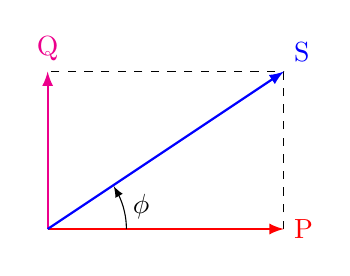
\begin{tikzpicture}
    \draw [dashed] (3,0) -- (3,2) -- (0,2);
    \draw [red,thick,-latex] (0,0) -- (3,0) node[right]{P};
    \draw [magenta,thick,-latex] (0,0) -- (0,2) node[above]{Q};
    \draw [blue,thick,-latex] (0,0) -- (3,2)node[above right]{S};
    \draw [-latex] (1,0) arc (0:33:1)node[midway,right]{$\phi$};
    \end{tikzpicture}
    \caption{Interprétation géométrique des quatre types de puissance dans le plan complexe.}
    \label{puissanceComp}
\end{figure}

La figure \ref{puissanceComp} donne les liens géométriques entre la puissance complexe $\overline{S}$ et les trois autres puissances. Mathématiquement, on a bien évidemment :
\begin{equation}
\overline{S} = P + jQ = Se^{j\phi}
\end{equation}

et
\begin{equation}
S^2 = P^2 + Q^2
\end{equation}

Le \textbf{bilan de puissances complexes} sur un circuit isolé est toujours nul. On peut aussi remarquer que la partie réelle et la partie imaginaire doivent aussi être nulles donc le bilan de puissance active et réactive doit aussi être nul.

\begin{equation}
\sum \overline{S} = 0 \Longrightarrow \sum P = 0 \; \; \; \mathrm{et} \sum Q = 0
\end{equation}

Finissons cette partie par noter que pour maximiser la puissance dissipée dans une charge $Z_L$ aux bornes d'une source en série avec une impédance équivalente $Z_S$, on doit choisir $Z_L$ = $Z_S^*$. Le rendement (le rapport entre la puissance dissipée dans $Z_L$ et celle fournie par la source) est alors de $\eta = 50\%$. Il n'est pas possible d'obtenir un rendement plus grand.

\section{Circuits triphasés}
L'avantage des circuits triphasés est, comme nous allons le voir, que la puissance consommée/fournie dans un circuit triphasé est constante même si les sources sont sinusoïdales. Un second avantage est que, comparé à 3 circuits indépendants, on utilise beaucoup moins de fils, ce qui est un avantage quand il s'agit de lignes de tension sur de grandes distances par exemple.
\subsection{Sources et charges triphasées}
\subsubsection*{Sources triphasées}
Une \textbf{source triphasée} est un ensemble de trois sources, généralement de tension, connectées en étoile (\textbf{Y}) ou en triangle($\Delta$) (voir figure \ref{sourceTri}). Ces trois sources sont sinusoïdales de même fréquence mais déphasées de $2 \pi / 3$. Si en outre leurs amplitudes sont égales, on parle de \textbf{source triphasée équilibrée}. On aura alors pour $V_1 + V_2 + V_3 = I_1 + I_2 + I_3 = 0$ (pour s'en convaincre, il suffit de tracer le diagramme phasoriel).


\begin{figure}[h]
	\centering
    \begin{circuitikz}[american]
    	\ctikzset{label/align = straight}
    	\draw (4,0) node[right]{S} to[V,l_=$e_1$,*-*] (2,2.82)node[above]{R} to[V,l_=$e_3$,-*] (0,0) node[left]{T} to[V,l_=$e_2$] (4,0); 
    	\draw (8,0.94) to[V=$e_1$,*-](6,0) node[left]{R};
    	\draw (8,0.94) to[V=$e_2$](8,2.82) node[above]{S};
    	\draw (8,0.94) to[V=$e_3$](10,0) node[right]{T};
    	\draw (8,0.94) node[right]{N};
    \end{circuitikz}
    \caption{Les deux types de source triphasée. A gauche la source triangle et à droite la source étoile.}
    \label{sourceTri}
\end{figure}

Pour passer d'un type de connexion à l'autre on utilise la relation\footnote{Petite démonstration (plus détaillée que "regarder le diagramme phasoriel") pour les motivés : pour y arriver, imaginons qu'on veuille passer d'une connexion étoile à une connexion triangle. Il suffit de calculer la tension aux bornes $V_{RS}$ (aussi appelée la tension de ligne, voir plus loin) qui vaut $V_R - V_S = e_1 - e_2$. Comme on ne s'intéresse pas au déphasage éventuel, il suffit de calculer le module de $e_1 - e_2 $. Considérons sans perte de généralité de module de $e_1$ et $e_2$ valant 1 et le déphasage de $e_1$ étant nul, on calcule alors $e_1 - e_2 = \cos(\omega t) - \cos (\omega t + 2 \pi /3) = (1+\frac{1}{2}) \cos(\omega t) + \frac{\sqrt{3}}{2} \sin(\omega t)$ et on trouve bien le facteur $\sqrt{(\frac{3}{2})^2 + (\frac{\sqrt{3}}{2})^2} = \sqrt{3}$, en utilisant la formule trigonométrique pour $\cos(a+b)$.} suivante concernant la valeur maximale/RMS des sources (on ne s'intéresse pas au changement de phase de celles-ci) :

\begin{equation}
e_{\Delta} = \sqrt{3} e_{Y}
\end{equation}

Attention, cette relation n'est valable que pour une source triphasée de tension équilibrée! Pour des sources de courants, il faut inverser la relation ($ \sqrt{3} I_{\Delta} = I_{Y}$).

\subsubsection*{Charges triphasées}
Les \textbf{charges triphasées} existent dans les mêmes configurations (on remplace les sources de la figure \ref{sourceTri} par des impédances. Par contre, la transformation ne se déroule pas de la même manière : il s'agit de la transformation "classique" triangle-étoile (qui est dans le formulaire, au cas où...) vue tout au début avec des résistances (qu'on étend maintenant aux impédances). Pour une charge triphasée équilibrée, on trouve simplement la relation :

\begin{equation}
Z_{\Delta} = 3 Z_{Y}
\end{equation}

\subsubsection*{Grandeurs de ligne et grandeurs de phase}
Les \textbf{grandeurs de ligne d'un circuit triphasé} sont les grandeurs que l'on peut mesures sur la ligne (les 'fils') entre la source et la charge, comme indiqué sur la figure \ref{grandeurLigne}. Elles sont particulièrement importantes : sauf mention contraire, c'est elles qui sont données.

\begin{figure}[h]
	\centering
    \includegraphics[scale=0.65]{grandeurLigne}
    \caption{Illustration des tensions et courants de ligne.}
    \label{grandeurLigne}
\end{figure}

Les \textbf{grandeurs de phase d'une source/charge triphasée} sont les tensions/courants à \textit{l'intérieur} d'une source/charge triphasée. Plus particulièrement, il s'agit de la tension des sources/sur les charges et des courants qui traversent ceux-ci. Il peut donc par exemple y avoir deux courants de phases différents au sein d'un même circuit triphasé, un associé à la source et un associé à la charge.

Le tableau suivant donne le lien entre grandeurs de ligne et de phase dans les deux cas de connexion (en négligeant les changements de phase). On retrouve logiquement les mêmes formules que pour les transformations de source, vu qu'on calcule au final les mêmes valeurs.
\begin{center}
    \begin{tabular}{ | l | l | l |}
    \hline
    Connexion  & \textbf{$\Delta$} & \textbf{Y} \\ \hline
    Tensions & $V_{ligne} = V_{phase}$ & $V_{ligne} = \sqrt{3}V_{phase}$  \\ \hline
    Courants & $\sqrt{3}I_{ligne} = I_{phase}$ & $I_{ligne} = I_{phase}$   \\ \hline
    \end{tabular}
\end{center}

\subsubsection*{Puissance dans un circuit triphasé}
Si $e_i$ et $i_i$ sont les tensions et courants de phase dans une charge triphasée, la puissance dissipée totale est $p(t) = \sum e_i(t)i_i(t)$. Dans le capitre sur la puissance, on a déjà démontré que $e(t)i(t) = P_{moy} + \cos(2 \omega t + \phi)$ à un déphasage près pour deux sources sinusoïdales. On peut montrer\footnote{Il s'agit d'une démonstration semblable à celle ou on montre que la somme des tensions d'une source triphasée est nulle.} que pour la somme des trois sinusoïdes s'annule pour tout t, et il reste dans la somme des trois puissances moyennes. La puissance dissipée dans la charge triphasée est donc constante et vaut :

\begin{equation}
P_{tri} = 3 P_{moy} = 3V_{eff}I_{eff}\cos(\phi)
\end{equation}

\subsection{Résoudre un circuit triphasé}
Pour résoudre un circuit triphasé, on essaye en général d'en extraire un circuit monophasé, plus facile à résoudre, comme indiqué dans la figure \ref{triMono}. Pour cela il faut premièrement transformer toutes les sources et charges en connexions étoile en utilisant les relations étoile-triangle présentées plus haut.

\begin{figure}[H]
	\centering
    \includegraphics[scale=0.65]{triToMono}
    \caption{Exemple de circuit monophasé extrait d'un circuit triphasé.}
     \label{triMono}
\end{figure}

Ensuite, une fois qu'on a extrait le circuit monophasé, on travaille dessus comme d'habitude. Il faut juste garder à l'esprit que le circuit est constitué de 3 circuits comme celui-ci, et que quand on parle de puissance dissipée par exemple il ne faut pas oublier de la multiplier par 3.

\todo[inline,color=blue]{exemple?}

\section{Mesures}
\subsection{Erreurs et incertitudes}
\subsubsection*{Erreurs}
Par définition, l'\textbf{erreur absolue} $e$ d'une mesure est la différence entre la \textbf{valeur vraie} $\xi$ et la \textbf{valeur mesurée} $x$. On peut distinguer deux composantes distinctes de cette erreur : la \textbf{composante systématique} $\delta$ (constante pour chaque mesure) et la \textbf{composante aléatoire} $\epsilon$.

\begin{equation}
e = x - \xi = \delta + \epsilon
\end{equation}

L'\textbf{erreur relative} $e_r$ donne l'importance relative de l'erreur absolue par rapport à la valeur réelle :

\begin{equation}
e_r = \frac{e}{\xi} = \frac{x - \xi}{\xi}
\end{equation}

Le problème c'est qu'en général on ne connait pas la vraie valeur $\xi$ (bah sinon ça sert à rien de faire la mesure) et on ne dispose que de $x$. On s'intéresse donc à la fiabilité d'une telle mesure $x$ : c'est là qu'intervient l'incertitude. Avant de passer à ce sujet, notons qu'on peut souvent éliminer l'erreur systématique $\delta$ par \textbf{étallonnage} : on prend une série de mesures dont on connait la valeur vraie en faisant varier la valeur de $\xi$ : le grand nombre de mesures permet de prendre la moyenne et de négliger $\epsilon$ : on trouve ensuite $\delta$ en observant un offset constant entre $x$ et $\xi$.

\subsubsection*{Incertitudes}
L'\textbf{incertitude} est une estimation des bornes maximales de l'erreur (qui dépendent des valeurs que $\epsilon$ peut prendre) : elle se traduit par un intervalle de valeurs. En faisant certaines hypothèses sur $\epsilon$ (et en négligeant $\delta$, qu'on aura pu éliminer par étallonage par exemple) cet intervalle est de la forme $[x - 2\sigma, x + 2\sigma]$ (par exemple $[1 - 0.2 V, 1 + 0.2 V]$. On est alors certain que la vraie valeur $\xi$ se situe avec une probabilité de $95\%$\footnote{Au Q5 tout cela deviendra probablement plus clair avec proba stat} dans cet intervalle. Cette valeur $2 \sigma$ est appelée l'\textbf{incertidue absolue} (l'incertude relative $ 2\sigma_r$ est définie de manière identique. On a aussi $\sigma_r = \sigma / \xi$).

\hspace{0pt} \\
Imaginons qu'on ait effectué plusieurs mesures A et B et qu'on ait caractérisé leurs incertutides absolues. Que valent les incertitudes absolues des opérations entre A et B? On suppose d'abord que les mesures A et B sont \textit{indépendantes}.
\begin{itemize}
\item \textbf{Addition/soustraction A $\pm$ B} pour une différence de tension par exemple. Dans ce cas, on a\footnote{Pour ceux qui ont déjà fait un peu de stats, on additionne non pas les écarts types $\sigma$ mais les variances $\sigma^2$. Mais ceci sort du cadre de ce cours.} :
\begin{equation}
\sigma_{AB} = \sqrt{\sigma_A^2 + \sigma_B^2}
\end{equation}

Si on a une mesure B très précise ($\sigma_B$ très petit), on voit que l'incertitude finale peut être très grande si A n'est pas précis : c'est la mesure la moins précise qui détermine la précisiondu résultat final.

\item \textbf{Multiplication/division A*B ou A/B}, pour un calcul de puissance par exemple.
On a alors :
\begin{equation}
\sigma_{AB} = \xi_A \xi_B \sqrt{(\frac{\sigma_A}{\xi_A})^2 + (\frac{\sigma_B}{\xi_B})^2}
\end{equation}

pour la multiplication (pour la division, il faut changer le facteur devant la racine par $\frac{\xi_A}{\xi_B}$) : on voit apparaitre les incertidues relatives dans la racine. Ici, c'est la plus grande incertitude relative qui domine.
\end{itemize}
\hspace{0pt} \\
Si les mesures A et B sont \textit{dépendantes}, on ne peut pas appliquer directement les formules ci-dessus. Par contre, on peut calculer les "valeurs extrêmes" du résultat en prenant les valeurs qui bornent les intervalles des mesures A et B qi donneront le plus grand et le plus petit résultat. On obtient ainsi un nouvel intervalle de valeurs comprenant la valeur vraie avec une probabilité de $95\%$; en écrivant ce nouvel intervalle sous une forme $[\xi_{AB} - 2 \sigma_{AB}, \xi_{AB} + 2 \sigma_{AB}]$, on peut déterminer la valeur de la nouvelle incertitude absolue $2 \sigma_{AB}$.

\subsection{Ponts de mesures}
Le principe des ponts de mesure est de se baser sur une comparaison plutôt que sur une mesure absolute, ce qui est beaucoup plus précis.
On pourra mesurer des impédances (exact à moins de 100ppm\footnote{Partie par million} près), ou des faibles variations (en fonction de la température etc.) d'impédance en comparant à une valeur standard (exact à quelques ppm près).

Les ponts de mesure ont deux objectifs distincts: \begin{itemize}
\item mesure d'une légère variation d'impédance par mesure de tension
\item mesure de la valeur absolue d'une impédance en en adaptant une autre pour annuler la tension mesurée
\end{itemize}

On prend pour exemple le pont de Wheatstone, comme visible à la figure \ref{pontmesures}. La mesure à effectuer sera la tension $V_{AB}$ indiquée. Pour un diviseur résistif, à droite sur cette même figure, il faudra également mesurer la tension $V_{AB}$.
\begin{figure}[h]
\centering
\includegraphics[width=.8\linewidth]{pontmesures}
\caption{Pont de Wheatstone et diviseur résistif}
\label{pontmesures}
\end{figure}
On résout le circuit du pont de Wheatstone (deux diviseurs de tension) pour trouver $V_{AB}$, ce qui donne
$$ H = \frac{V_{AB}}{V_S} = \frac{R_{AY}}{R_{AX} + R{AY}} - \frac{R_{BY}}{R_{BX} + R{BY}}.$$
L'objectif numéro 1, de mesurer une légère variation, s'exprime ainsi: $R_{AX} = (1+\alpha)R$ et $R_{AY} = R_{BX} = R_{BY} = R.$ On a alors $ H = -\frac{\alpha}{2(2+\alpha)}$. Le deuxième objectif est rempli quand $V_{AB} = 0 = H$, et on a alors effectivement $R_{AX} = R_{AY}$.

Pour comparer cette mesure à celle d'un simple diviseur résistif, revenons à la figure \ref{pontmesures}. Pour $V_s = 10V$ et $\alpha=\pm 1\%$, la gamme de mesures nécessaire pour le pont de Wheatstone est de $\pm 50mV$, alors qu'elle est de 0 à 10V pour le diviseur résistif. On observera en sortie $V_M \approx \pm 25mV$ contre $V_M \approx 5\pm 25mV$. Avec des voltmètres d'une imprécision de 1\%, cela donne une précision de $1mV$ pour le pont de Wheatstone et de $100mV$ pour le diviseur résistif.

Pour les ponts de mesure d'impédances, il faut garder à l'esprit que deux impédances sont égales si leur norme et phase sont égales.



%\subsection{Amplificateur de mesure : exemple d'implémentation} % est-ce vraiment utile???

\end{document}
